% ********** Rozdział 4 **********
\chapter{Prezentacja warstwy użytkowej projektu}

\section{Opis warstwy użytkowej}
Warstwa użytkowa w omawianej aplikacji została zaimplementowana 
w postaci konsolowego programu (\texttt{Program.cs}). Użytkownik wchodzi w interakcję 
z systemem poprzez menu wyświetlane w konsoli, w którym dostępne są następujące opcje:
\begin{figure}[H] 
    \centering
    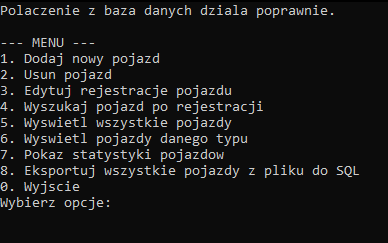
\includegraphics[width=1\textwidth]{ManuGlowne.png}
    \caption{Menu główne aplikacji}
    \label{fig:moj_obrazek}
\end{figure}
\begin{itemize}
    \item \textbf{Dodawanie nowego pojazdu} -- użytkownik wprowadza dane pojazdu (marka, model, rok itp.), 
    a program wywołuje odpowiednie metody warstwy dostępowej do bazy (np. \texttt{DodajNowyPojazd}).
    \begin{figure}[H] 
        \centering
        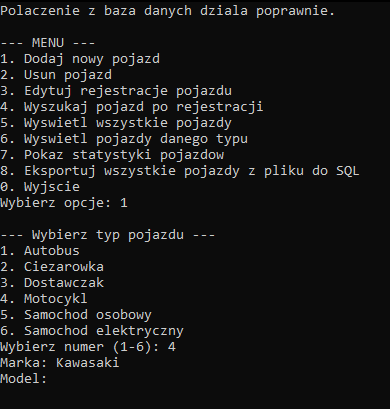
\includegraphics[width=1\textwidth]{Dodawanie.png}
        \caption{Dodawanie pojazdu}
        \label{fig:moj_obrazek}
    \end{figure}
    \item \textbf{Usuwanie pojazdu} -- użytkownik podaje numer rejestracyjny, a aplikacja usuwa pojazd 
    z bazy plikowej i bazy SQL.
    \begin{figure}[H] 
        \centering
        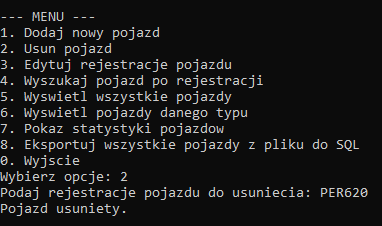
\includegraphics[width=1\textwidth]{Usuwanie.png}
        \caption{Usuwanie pojazdu}
        \label{fig:moj_obrazek}
    \end{figure}
    \item \textbf{Edycja rejestracji} -- umożliwia zmianę numeru rejestracyjnego istniejącego pojazdu.
    \begin{figure}[H] 
        \centering
        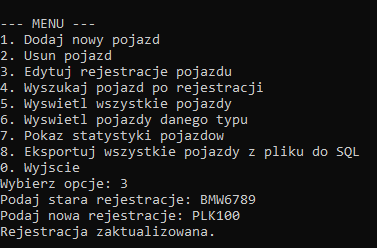
\includegraphics[width=1\textwidth]{Rejestracja.png}
        \caption{Edycja rejestracji}
        \label{fig:moj_obrazek}
    \end{figure}
    \item \textbf{Wyszukiwanie pojazdu} -- na podstawie rejestracji program wyświetla informacje 
    o odnalezionym pojeździe (lub komunikat o braku pojazdu).
    \begin{figure}[H] 
        \centering
        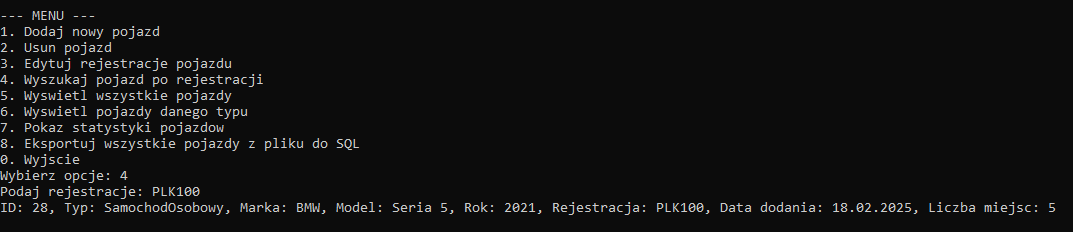
\includegraphics[width=1\textwidth]{WyszukiwanieRejestracja.png}
        \caption{Wyszukiwanie pojazdu po numerze rejestracyjnym}
        \label{fig:moj_obrazek}
    \end{figure}
    \item \textbf{Wyświetlanie pojazdów} -- aplikacja pobiera listę wszystkich pojazdów z warstwy dostępowej 
    i prezentuje je w konsoli.
    \begin{figure}[H] 
        \centering
        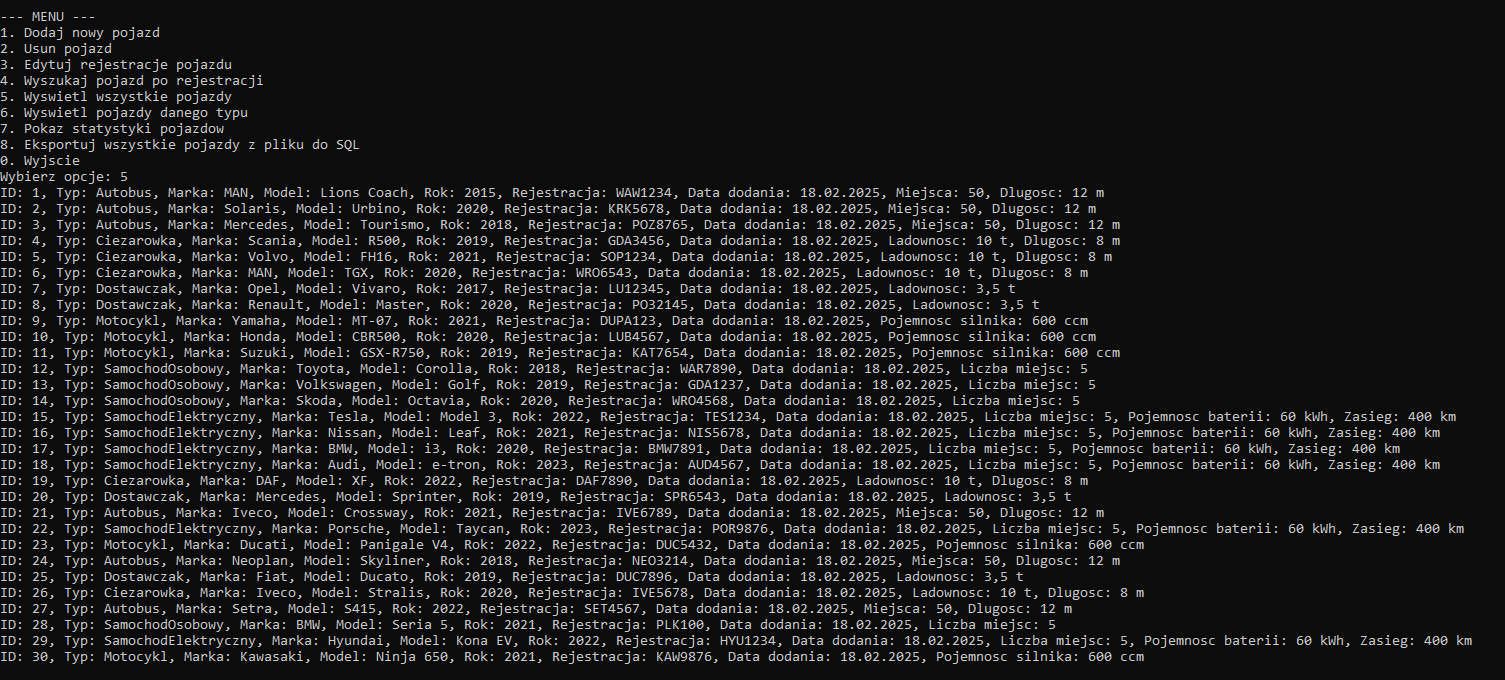
\includegraphics[width=1\textwidth]{Wyswietlanie wszyskiego.png}
        \caption{Wyświetlanie wszystkich pojazdów}
        \label{fig:moj_obrazek}
    \end{figure}
    \item \textbf{Wyświetlanie pojazdów danego typu} -- użytkownik wybiera typ (np. \textit{Autobus}, 
    \textit{Ciezarowka}, \textit{Motocykl}), a program wyświetla pasujące rekordy.
    \begin{figure}[H] 
        \centering
        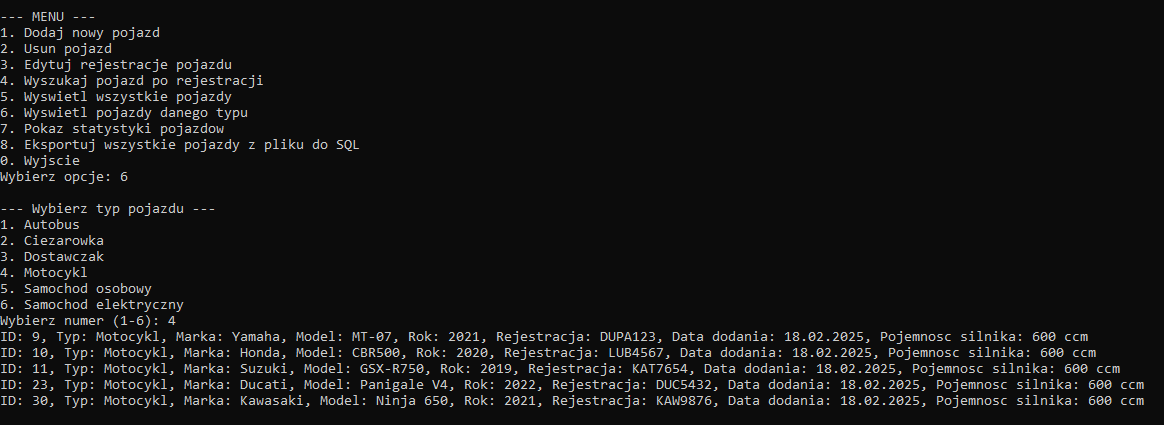
\includegraphics[width=1\textwidth]{DanyTyp.png}
        \caption{Wyswietlanie danego typu pojazdow}
        \label{fig:moj_obrazek}
    \end{figure}
    \item \textbf{Statystyki} -- pozwala na wyświetlenie informacji statystycznych (np. liczba pojazdów 
    w każdej kategorii).
    \begin{figure}[H] 
        \centering
        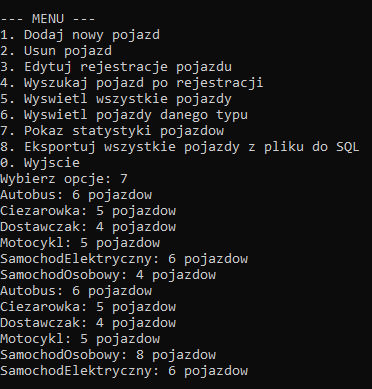
\includegraphics[width=1\textwidth]{Statystyki.png}
        \caption{Statystyki pojazdów}
        \label{fig:moj_obrazek}
    \end{figure}
    \item \textbf{Eksport do SQL} -- umożliwia przeniesienie danych z bazy plikowej do bazy SQL 
    (z zachowaniem walidacji).
    \begin{figure}[H] 
        \centering
        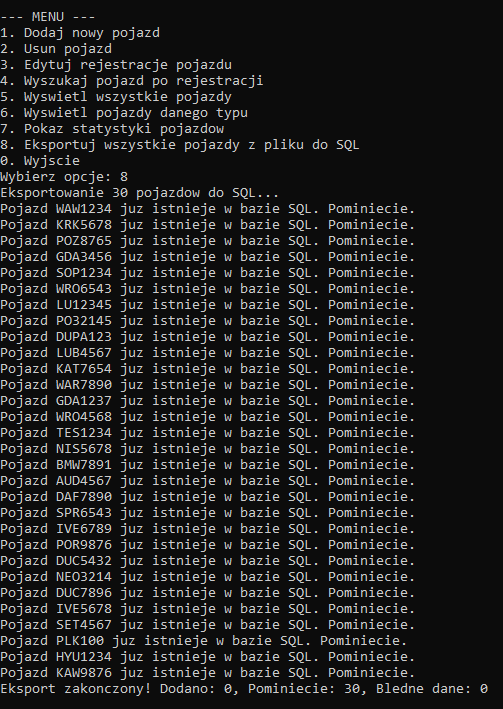
\includegraphics[width=1\textwidth]{Eksport.png}
        \caption{Eksport danych do SQL}
        \label{fig:moj_obrazek}
    \end{figure}
\end{itemize}

\subsection{Sposób działania}
Cała komunikacja z użytkownikiem odbywa się w pętli \texttt{while}, która wyświetla menu 
i w zależności od wybranej opcji wywołuje konkretne metody warstwy dostępowej. 
Dzięki temu warstwa użytkowa jest odpowiedzialna wyłącznie za:
\begin{enumerate}
    \item Pobieranie danych wejściowych od użytkownika,
    \item Wywoływanie metod z warstwy logiki/baz danych (np. \texttt{DodajPojazd}, \texttt{UsunPojazd}),
    \item Prezentację wyników w konsoli (np. listy pojazdów, komunikaty o błędach).
\end{enumerate}

\subsection{Zalety podejścia}
\begin{itemize}
    \item \textbf{Oddzielenie logiki biznesowej od interfejsu} -- kod obsługujący dane i bazę jest w odrębnych klasach, 
    co ułatwia modyfikacje i testy.
    \item \textbf{Łatwa rozbudowa} -- w przyszłości można zastąpić interfejs konsolowy np. interfejsem graficznym, 
    bez konieczności modyfikowania metod logiki lub bazy danych.
    \item \textbf{Przejrzystość} -- menu konsolowe jest intuicyjne w obsłudze, a kolejne opcje (dodawanie, usuwanie, 
    wyszukiwanie) są jasno wyodrębnione.
\end{itemize}

\section{Podsumowanie}
Warstwa użytkowa w postaci aplikacji konsolowej stanowi prosty, ale skuteczny sposób 
na interakcję z systemem \textbf{ZarządzaniePojazdami}. Dzięki czytelnej strukturze menu 
oraz wywoływaniu metod z warstwy logiki i dostępu do danych, użytkownik może w łatwy sposób 
dodawać, usuwać, modyfikować i przeglądać pojazdy w bazie.



